

The following games were created from the saddle point problems of rational polynomials studied by \textcite{zhou.wang.ea:saddle}. The utility functions are not continuous on the whole strategy set as the divisor often vanishes on the boundary.

\begin{game}\label{ex.zhou19.5.1}

A two-player zero-sum game in $3 \times 3$ variables on the simplex
\[
x_i \in \Delta^{2} \quad \forall i \in \{1,2\}.
\]
The rational utility function \cite[Example~5.1]{zhou.wang.ea:saddle} is given by
\[
u_1(x_1, x_2) =
\frac{
- \sum_{i=1}^{3} \sum_{j=1}^{3} x_{1i}^2 x_{2j}^2 + \sum_{i=1}^{3} \sum_{\substack{j=1 \\ i \ne j}}^{3} (x_{1i} x_{1j} + x_{2i} x_{2j})
}{
x_{11} + x_{12} + x_{22} + x_{23}
}
\]
This game has two pure Nash equilibria:
\begin{align*}
\text{NE}_1: &x_1^\star \approx (0.3165, 0.3165, 0.3670),\,x_2^\star = (0, 1, 0),\\
\text{NE}_2: &x_1^\star \approx (0.3165, 0.3165, 0.3670),\,x_2^\star = (0, 0, 1).
\end{align*}
\end{game}

\begin{game}\label{ex.zhou19.5.2.ii}
A two-player zero-sum game in $3 \times 3$ variables on the hypercube
\[
x_i \in [-1,1]^3 \quad \forall i \in \{1,2\}.
\]
The rational utility function \cite[Example~5.2 (ii)]{zhou.wang.ea:saddle} is given by
\[
u_1(x_1, x_2) =
\frac{
- \sum_{i=1}^{3} x_{1i}^2 + \sum_{i=1}^{3} x_{2i}^2
}{
\sum_{i=1}^{3} x_{2i}^2 - \sum_{i=1}^{3} x_{1i}^2 + 3
}
\]
This game has a pure Nash equilibrium at
\begin{align*}
x_1^\star = (0, 0, 0),\, x_2^\star = (0, 0, 0).
\end{align*}
\end{game}

\begin{game}\label{ex.zhou19.5.4.i}
A zero-sum 2-player game in $3 \times 3$ variables on the nonnegative orthant
\[
x_i \in \mathbb{R}^3_+ \quad \forall i \in \{1,2\}
\]
with the utility function \cite[Example~5.4 (i)]{zhou.wang.ea:saddle}
\[
u_1(x_1, x_2) =
\frac{
- x_{11}^4 - x_{12}^4 - x_{13}^4 + x_{21}^4 + x_{22}^4 + x_{23}^4
}{
x_{11} + x_{21} + 1
}
\]
The game has a pure Nash equilibrium:
\begin{align*}
x_1^\star \approx (0.0015, 0.0015, 0.0015), \\
x_2^\star \approx (0.0015, 0.0015, 0.0015).
\end{align*}
\end{game}


\begin{game}\label{ex.zhou19.5.5.i}

A two-player zero-sum game in $2 \times 2$ variables on the ball
\[
x_i \in \left\{ z \in \mathbb{R}^2 \,\middle|\, \norm{z} \leq 1  \right\} \quad \forall i \in \{1,2\}
\]
The rational utility function \cite[Example~5.5 (i)]{zhou.wang.ea:saddle} is
\[
u_1(x_1, x_2) =
\frac{
- x_{11}^2 - x_{12}^2 + 3 x_{11} x_{12} + x_{21}^2 + x_{22}^2 - x_{21} x_{22}
}{
x_{11} x_{21} + 1
}
\]
This game has no pure Nash equilibria.
\end{game}

\begin{game}\label{ex.zhou19.5.5.ii}

A two-player zero-sum game in $3 \times 3$ variables on the ball
\[
x_i \in \left\{ z \in \mathbb{R}^3 \,\middle|\, \norm{z} \leq 1  \right\} \quad \forall i \in \{1,2\}
\]
The rational utility function \cite[Example~5.5 (ii)]{zhou.wang.ea:saddle} is
\[
u_1(x_1, x_2) =
\frac{
- x_{11}^2 x_{21} - 2 x_{12}^2 x_{22} - 3 x_{13}^2 x_{23} + x_{11} + x_{12} + x_{13}
}{
x_{11} x_{21} + 1
}
\]
This game has a pure Nash equilibrium at
\begin{align*}
x_1^\star \approx (0.4730, 0.4476, 0.3416),\, x_2^\star \approx (0.6708, 0.5585, 0.4879).
\end{align*}
\end{game}

\begin{game}\label{ex.zhou19.5.6.i}

A two-player zero-sum game in $3 \times 3$ variables on the sphere
\[
x_i \in \left\{ z \in \mathbb{R}^3 \,\middle|\, \norm{z} = 1  \right\} \quad \forall i \in \{1,2\}
\]
The rational utility function \cite[Example~5.6 (i)]{zhou.wang.ea:saddle} is
\[
u_1(x_1, x_2) =
\frac{
- \sum_{i=1}^{3} (x_{1i}^3 + x_{2i}^3) - 2 (x_{11} x_{12} x_{21} x_{22} + x_{11} x_{13} x_{21} x_{23} + x_{12} x_{13} x_{22} x_{23})
}{
x_{11} - x_{21} + 1
}
\]
The game has no pure NE.
\end{game}

\begin{game}\label{ex.zhou19.5.6.ii}

A two-player zero-sum game in $3 \times 3$ variables on the sphere
\[
x_i \in \left\{ z \in \mathbb{R}^3 \,\middle|\, \norm{z} = 1  \right\} \quad \forall i \in \{1,2\}
\]
The rational utility function \cite[Example~5.6 (ii)]{zhou.wang.ea:saddle} is
\[
u_1(x_1, x_2) =
\frac{
- \sum_{i=1}^{3} (x_{1i}^2 + x_{2i}^2 - x_{1i} - x_{2i})
}{
x_{13} + x_{22} + 2
}
\]
This game has a pure Nash equilibrium at
\begin{align*}
x_1^\star \approx (0.4082, 0.4082, 0.8165),\, x_2^\star \approx (−0.4082, −0.8165, −0.4082).
\end{align*}
\end{game}

\begin{game}\label{ex.zhou19.5.7.i}

A two-player zero-sum game in $3 \times 2$ variables on the intersection of the nonnegative orthant and the n-sphere
\begin{align*}
x_1 &\in \left\{ z \in \mathbb{R}^3_+ \,\middle|\, \norm{z} = 1  \right\} \\
x_2 &\in \left\{ z \in \mathbb{R}^2_+ \,\middle|\, \norm{z} = 1  \right\}
\end{align*}
The rational utility function is
\[
u_1(x_1, x_2) =
\frac{
- \sum_{i=1}^{3} (x_{1i}^2 - x_{1i}) - \sum_{i=1}^{2} (x_{2i} - x_{2i}^2)
}{
x_{11}^2 - x_{21}^2 + 1
}
\]
The utility has a discontinuity at the boundary of $x_1$ when $x_{21} = 1$. \textcite[Example~5.7 (i)]{zhou.wang.ea:saddle} report that this game has no saddle point, although we found the following pure $\epsilon$-NE (with $\epsilon < 10^{-8}$):
\begin{align*}
x_1^\star \approx (0.4351314094, 0.6366555805, 0.6366555805),\, x_2^\star \approx (0.5255286571, 0.8507758992).
\end{align*}
We also show this game reprojected in polar coordinates in \cref{ex.zhou19.5.7.i.polar}, where we recover the same solution.
\end{game}

\begin{game}\label{ex.zhou19.5.7.i.polar}
A two-player zero-sum game in $3 \times 2$ variables on the intersection of the nonnegative orthant and the n-sphere in polar coordinates
\begin{align*}
x_1 &\in \left[0,\frac{\pi}{2} \right]^2 \\
x_1 &\in \left[0,\frac{\pi}{2} \right]
\end{align*}
The utility function is
\[
u_1(x_1, x_2) = \upsilon\left(\bigl[\sin(x_{11}) \cos(x_{12}), \sin(x_{11}) \sin(x_{12}), \cos(x_{11})\bigr], \bigl[\cos(x_{21}), \sin(x_{21}) \bigr] \right)
\]
where
\[
\upsilon(z_1, z_2) = \frac{
- \sum_{i=1}^{3} (z_{1i}^2 - z_{1i}) - \sum_{i=1}^{2} (z_{2i} - z_{2i}^2)
}{
z_{11}^2 - z_{21}^2 + 1
}
\]
This example is the polar coordinate reformulation of the example by \textcite[Example~5.7 (i)]{zhou.wang.ea:saddle}. Despite containing a discontinuity at the boundary of $x_1$ when $x_{21}=0$ the game has the pure $\epsilon$-NE shown in \cref{fig:ex.polar.br}:
\begin{align*}
x_1^\star &\approx (0.8813, 0.9716),\\
x_2^\star &\approx 1.0175.
\end{align*}
\end{game}


\begin{figure}
\centering
\begin{minipage}{0.4\textwidth}
\centering
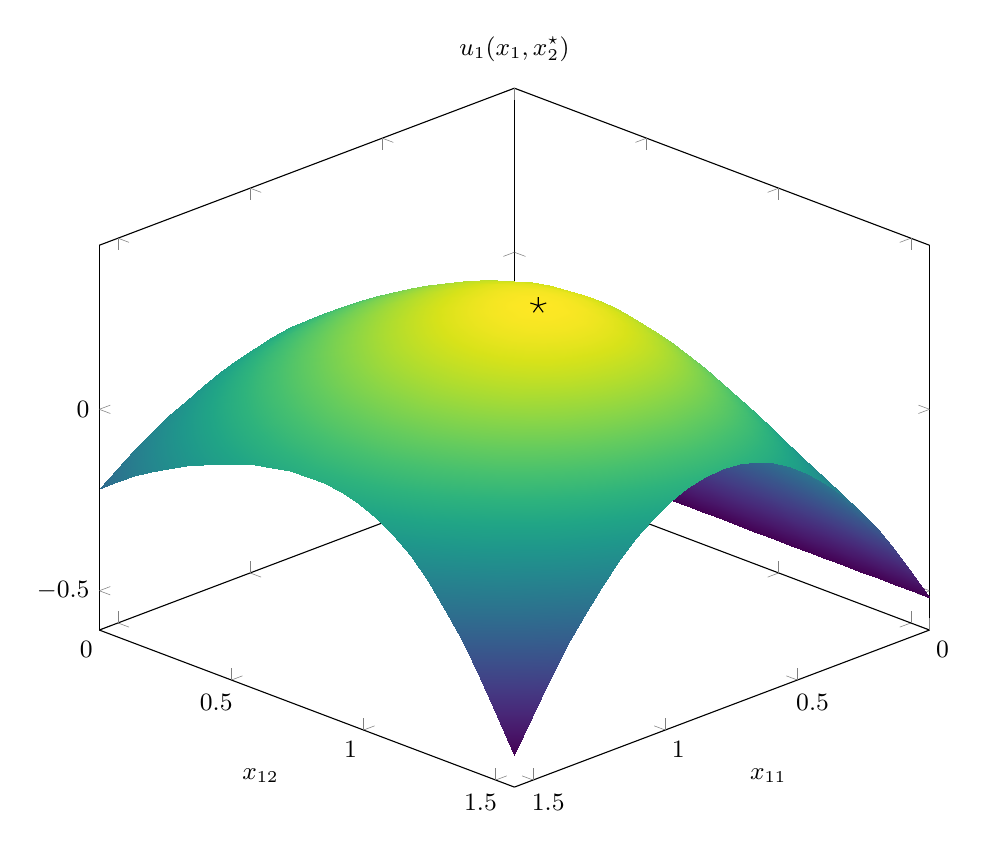
\begin{tikzpicture}
\begin{axis}[
    font=\small,
    domain=0:1.5707963267948966,
    y domain=0:1.5707963267948966,
    xlabel=$x_{11}$,
    ylabel=$x_{12}$,
    title={$u_1(x_1,x_2^\star)$},
    colormap/viridis,
    view={135}{30},
    mesh/ordering=y varies,
    width=\textwidth,
]
\addplot3[
    surf,
    shader=interp,
]
{-((0.376306020901492 - cos(deg(x)) - sin(deg(x))*sin(deg(y)) - sin(deg(x))*cos(deg(y)) + cos(deg(x))^2 + (sin(deg(x))^2)*(sin(deg(y))^2) + (sin(deg(x))^2)*(cos(deg(y))^2)) / (0.7238156036862534 + (sin(deg(x))^2)*(cos(deg(y))^2)))};
\addplot3[
    only marks,
    mark=star,
    color=black,
    mark size=3,
]
coordinates {(0.8812945920343842, 0.9716157415160604, 0.36372376459410616)};
\end{axis}
\end{tikzpicture}
\end{minipage}%
\hspace{1em}
\begin{minipage}{0.4\textwidth}
\centering
\begin{tikzpicture}
\begin{axis}[
    font=\small,
    domain=0:1.5707963267948966,
    xlabel=$x_{21}$,
    title={$u_2(x_1^\star,x_2)$},
    width=0.9\textwidth,
    colormap/viridis,
]
\addplot[
    thick,
]
{(-0.7084434199966159 + sin(deg(x)) + cos(deg(x)) - (sin(deg(x))^2) - (cos(deg(x))^2)) /
 (1.1893427638066412 - (cos(deg(x))^2))};
\addplot[
    only marks,
    mark=star,
    color=black,
    mark size=3,
]
coordinates {(1.0174554472964583, -0.36372376459410616)};
\end{axis}
\end{tikzpicture}
\end{minipage}
\caption{The best-response curves of both players at the $\epsilon$-NE of \cref{ex.zhou19.5.7.i.polar}.}
\label{fig:ex.polar.br}
\end{figure}


\begin{game}\label{ex.zhou19.5.7.ii}
A two-player zero-sum game in $3 \times 3$ variables on the intersection of the nonnegative orthant and the sphere
\[
x_i \in \left\{ z \in \mathbb{R}^3_+ \,\middle|\, \norm{z} = 1  \right\} \quad \forall i \in \{1,2\}
\]
with the utility function \cite[Example~5.7 (ii)]{zhou.wang.ea:saddle}
\[
u_1(x_1, x_2) =
\frac{
- \sum_{i=1}^{3} (x_{1i} - 1)^2 - \sum_{i=1}^{3} (x_{2i} - 1)^2
}{
x_{11}^2 - x_{21}^2 + 1
}
\]
The game has the pure NE
\begin{align*}
x_1^\star \approx (0.9519, 0.2167, 0.2167),\, x_2^\star \approx (1, 0, 0).
\end{align*}
\end{game}

\begin{game}\label{ex.zhou19.5.8.i}
A general-sum 2-player game in $3 \times 3$ variables with no constraints
\[
x_i \in \mathbb{R}^3 \quad \forall i \in \{1,2\}.
\]
with the utility function \cite[Example~5.8 (i)]{zhou.wang.ea:saddle}
\[
u_1(x_1, x_2) =
\frac{
- x_{11}^2 - x_{12}^2 - x_{13}^2 - x_{21}^2 - x_{22}^2 + x_{11} + x_{12}
}{
x_{11}^2 + x_{23}^2 + 1
}
\]
The game has a pure Nash equilibrium:
\begin{align*}
x_1^\star \approx (0.3508, 0.5000, 0.0000), \\
x_2^\star \approx (0.0000, 0.0000, 0.0000).
\end{align*}
\end{game}

\begin{game}\label{ex.zhou19.5.9.i}
A zero-sum 2-player game in $3 \times 3$ variables subject to the constraints
\[
x_i \in \left\{z \in \mathbb{R}^3 \,\middle|\, z_1 \geq 0, z_1z_2 \geq 1, z_2z_3 \geq 1 \right\} \quad \forall i \in \{1,2\}
\]
which define a non-compact set. The utility function \cite[Example~5.9 (i)]{zhou.wang.ea:saddle} is
\[
u_1(x_1, x_2) =
\frac{
- \sum_{i=1}^{3} (x_{1i}^2 - x_{1i} + x_{2i} - x_{2i}^2)
}{
x_{11}^2 + x_{21}^2 + 1
}
\]
The game has a pure Nash equilibrium:
\begin{align*}
x_1^\star \approx (0.8914, 1.1219, 0.8914), \\
x_2^\star \approx (0.8914, 1.1219, 0.8914).
\end{align*}
\end{game}


\begin{game}\label{ex.zhou19.5.9.ii}
A general-sum 2-player game in $3 \times 3$ variables subject to the constraints
\[
x_i \in \left\{z \in \mathbb{R}^3 \,\middle|\, z_1 \geq 0, z_1z_2 \geq 1, z_2z_3 \geq 1 \right\} \quad \forall i \in \{1,2\}
\]
which define a non-compact set. The utility function \cite[Example~5.9 (ii)]{zhou.wang.ea:saddle} is
\[
u_1(x_1, x_2) =
\frac{
- x_{11}^4 - x_{12}^4 + x_{21}^4 + x_{22}^4 - x_{11} x_{13} - x_{21} x_{23}
}{
x_{13}^2 + x_{23}^2 + 1
}
\]
The game has a pure Nash equilibrium:
\begin{align*}
x_1^\star \approx (0.9230, 1.0834, 2.8239), \\
x_2^\star \approx (1.0459, 0.9561, 1.3804).
\end{align*}
\end{game}


